\documentclass[12pt]{article}
\usepackage{amsthm,amssymb,amsmath,amsfonts}
\usepackage[a4paper, top=25mm, bottom=30mm, left=25mm, right=25mm]{geometry}
\usepackage[pagebackref=false,colorlinks,linkcolor=black,citecolor=black]{hyperref}
\usepackage[nameinlink]{cleveref}
 \AtBeginDocument{%
    \crefname{equation}{برابری}{equations}%
    \crefname{chapter}{فصل}{chapters}%
    \crefname{section}{بخش}{sections}%
    \crefname{appendix}{پیوست}{appendices}%
    \crefname{enumi}{مورد}{items}%
    \crefname{footnote}{زیرنویس}{footnotes}%
    \crefname{figure}{شکل}{figures}%
    \crefname{table}{جدول}{tables}%
    \crefname{theorem}{قضیه}{theorems}%
    \crefname{lemma}{لم}{lemmas}%
    \crefname{corollary}{نتیجه}{corollaries}%
    \crefname{proposition}{گزاره}{propositions}%
    \crefname{definition}{تعریف}{definitions}%
    \crefname{result}{نتیجه}{results}%
    \crefname{example}{مثال}{examples}%
    \crefname{remark}{نکته}{remarks}%
    \crefname{note}{یادداشت}{notes}%
    \crefname{observation}{مشاهده}{observations}%
    \crefname{algorithm}{الگوریتم}{algorithms}%
    \crefname{cproof}{برهان}{cproofs}%
}

\usepackage{tikz}
\usepackage{graphicx}
\usepackage{booktabs}
\usepackage{color}
\usepackage{graphicx}
\usepackage{subcaption}

\usepackage{setspace}
\doublespacing

\usepackage{titletoc}
\usepackage{tocloft}
\usepackage{enumitem}
\usepackage{amsmath, amssymb}
\usepackage{algorithm}
\usepackage[noend]{algorithmic}
\renewcommand{\algorithmicrequire}{\textbf{Input:}}
\renewcommand{\algorithmicensure}{\textbf{Output:}}

\usepackage{tabularx}
\makeatletter
\newcommand{\multiline}[1]{%
  \begin{tabularx}{\dimexpr\linewidth-\ALG@thistlm}[t]{@{}X@{}}
    #1
  \end{tabularx}
}
\makeatother

\usepackage{float}
\usepackage{verbatim}
\makeindex
\usepackage{sectsty}
\usepackage{xepersian}
\SepMark{-}
\settextfont[Scale=1.2,Path=fonts/,BoldFont=B Nazanin Bold.ttf]{B Nazanin.ttf}
\setlatintextfont{Times New Roman}
\renewcommand{\labelitemi}{$\bullet$}

\theoremstyle{definition}
\newtheorem{definition}{تعریف}[section]
\newtheorem{remark}[definition]{نکته}
\newtheorem{note}[definition]{یادداشت}
\newtheorem{example}[definition]{نمونه}
\newtheorem{question}[definition]{سوال}
\newtheorem{remember}[definition]{یاداوری}
\newtheorem{observation}[definition]{مشاهده}
\theoremstyle{theorem}
\newtheorem{theorem}[definition]{قضیه}
\newtheorem{lemma}[definition]{لم}
\newtheorem{proposition}[definition]{گزاره}
\newtheorem{corollary}[definition]{نتیجه}
\newtheorem*{cproof}{برهان}




\begin{document}
\fontsize{12pt}{14pt}\selectfont

\begin{minipage}{0.1\textwidth}

\includegraphics[width=3cm]{etc/IUST}
\end{minipage}%
\hfill%
\begin{minipage}{0.6\textwidth}\centering
\fontsize{13pt}{13pt}\selectfont
به‌ نام خدا \\
\textbf{درس یادگیری عمیق} \\
\textbf{تمرین سری ششم}\\
استاد درس : دکتر محمدرضا محمدی \\
دستیاران :  مهدی خورشا، سید محمد موسوی،\\ امیرحسین نمازی
\\
\vspace{0.25cm}
\begingroup
\fontsize{11pt}{11pt}\selectfont
دانشگاه علم و صنعت ایران، دانشکده مهندسی کامپیوتر \\
نیمسال دوم تحصیلی 1403 - 1404 \\
\endgroup
\end{minipage}%
\hfill%
\begin{minipage}{0.1\textwidth}

\end{minipage}

\vspace{0.5cm}

\noindent\rule{\textwidth}{1pt}

\centering {\fontsize{18}{22}\selectfont \textbf{مهلت تحویل : 1404/05/05 }}\\
{\fontsize{14}{22}\selectfont \textbf{لطفا به نکات موجود در سند قوانین انجام و تحویل تمرین ها دقت فرمایید. }}

\begin{enumerate}

    \section*{سوالات تئوری}
    \item 
\includegraphics[width=1cm]{figs/Forbidden_AI.jpg}
    روش‌های پیشرفته‌ی یادگیری ماشین خودکار مانند جستجوی معماری عصبی (\lr{NAS}) و \lr{AutoAugment}  برای خودکارسازی جنبه‌های پیچیده طراحی مدل توسعه یافته‌اند. اصول اصلی این روش‌ها را توضیح دهید و موارد زیر را بررسی کنید. برای هریک از ۲ روش ذکر شده، موارد ذیل را به صورت جداگانه مورد بحث قرار دهید:(۲۰ نمره)
    
    \begin{enumerate}
        \item نحوه تعریف مسئله‌ی خودکارسازی توسط هر تکنیک
        \item سازوکارها یا ساختارهای کنترلی مورد استفاده (مثل \lr{Controller-Trainer}، \lr{sub-policies})
        \item چالش‌های مرتبط با پیچیدگی فضای جستجو و هزینه محاسباتی
        \item نقش یادگیری تقویتی (\lr{RL})، بهینه‌سازی بیزی و تطابق چگالی در حل این چالش‌ها
        \item ذکر نمونه‌ها یا نسخه‌های خاص هر روش (در صورت وجود)
    \end{enumerate}

    \textcolor{blue}{
        \textbf{جستجوی معماری عصبی (\lr{NAS})}
        \begin{itemize}
            \item تعریف مسئله\\
                \lr{NAS} فرآیند طراحی خودکار معماری شبکه عصبی را به‌صورت مسئله‌ای بهینه‌سازی فرموله می‌کند که هدف آن یافتن معماری‌ای با بیشترین عملکرد (مثل دقت بالا) است.
            \item سازوکار کنترل\\
                ساختار متداول در \lr{NAS}، مدل کنترل‌گر-آموزش‌دهنده (\lr{Controller-Trainer}) است:
                \begin{itemize}
                    \item کنترل‌گر (معمولاً یک شبکه بازگشتی) معماری جدیدی را تولید می‌کند.
                    \item این معماری توسط آموزش‌دهنده (\lr{Trainer}) آموزش داده می‌شود.
                    \item دقت مدل حاصل بر مجموعه اعتبارسنجی به‌عنوان پاداش در نظر گرفته می‌شود.
                    \item پارامترهای کنترل‌گر بر اساس این پاداش با استفاده از \lr{RL} به‌روزرسانی می‌شوند.
                \end{itemize}
            \item چالش‌ها\\
                فضای جستجوی معماری بسیار بزرگ و پیچیده است و آموزش هر معماری هزینه زیادی دارد.
            \item حل چالش‌ها با \lr{RL} و بهینه‌سازی\\
                از یادگیری تقویتی (\lr{RL}) برای آموزش کنترل‌گر استفاده می‌شود تا معماری‌های بهتری تولید کند.
            \item نمونه‌ها و نسخه‌ها\\
                \begin{itemize}
                    \item \textbf{جستجوی سلولی:} بسیاری از روش‌ها ابتدا یک ساختار پایه (\lr{Cell}) را جستجو می‌کنند و سپس شبکه را از روی آن می‌سازند.
                    \item \textbf{\lr{EfficientNet}:} با الهام از \lr{MnasNet}، بهینه‌سازی چندهدفه انجام می‌دهد (تعادل بین دقت و هزینه محاسباتی). معیار آن:
                    $$
                    ACC \times \left( \frac{FLOPS}{T} \right)^w
                    $$
                    \item \textbf{\lr{DARTS}:} با وزن‌دهی پیوسته به عملیات‌ها و حذف اتصالات ضعیف، فضای جستجو را به‌صورت قابل تفکیک و قابل مشتق‌گیری مدل می‌کند.
                \end{itemize}
        \end{itemize}\\
        \textbf{\lr{AutoAugment}}
        \begin{itemize}
            \item تعریف مسئله\\
                هدف \lr{AutoAugment} یافتن بهترین روش‌های افزایش داده (\lr{Data Augmentation}) برای بهبود عملکرد مدل است.
            \item سازوکار کنترلی\\
                \begin{itemize}
                    \item هر عملیات افزایش داده دارای سه پارامتر است: نوع عملیات (مثل چرخش، کشش)، احتمال اعمال، و شدت عملیات (\lr{intensity}).
                    \item یک \lr{sub-policy} مجموعه‌ای از چند عملیات است که روی یک نمونه داده اجرا می‌شود.
                    \item یک سیاست از چند زیرسیاست \lr{sub-policy} تشکیل شده که یکی از آن‌ها در هر تکرار آموزش انتخاب می‌شود.
                \end{itemize}
            \item چالش‌ها\\
                فضای جستجو بسیار بزرگ است (برای مثال، $2.9 \times 10^{32}$ حالت ممکن برای ۵ زیرسیاست با ۱۶ عملیات و ۱۰ شدت و احتمال).
            \item حل چالش‌ها با (\lr{RL}, \lr{Bayesian Optimization}, \lr{Density Matching})\\
                \begin{itemize}
                    \item \lr{AutoAugment} اولیه از یادگیری تقویتی (\lr{RL}) استفاده می‌کرد.
                    \item \lr{Fast AutoAugment} برای کاهش هزینه محاسباتی، از بهینه‌سازی بیزی (\lr{BO}) استفاده می‌کند.
                    \item همچنین، از تطبیق چگالی (\lr{Density Matching}) استفاده می‌کند تا داده‌های افزایش‌یافته توزیعی مشابه داده اصلی داشته باشند.
                \end{itemize}
        \end{itemize}
    }
    \item 
\includegraphics[width=1cm]{figs/Forbidden_AI.jpg}
    \begin{enumerate}
            \item ماتریس \lr{W} زیر را در نظر بگیرید. ابتدا تعریف کنید که مرتبه (\lr{rank}) یک ماتریس چیست و چه مفهومی دارد سپس مرتبه ماتریس \lr{W} را به صورت دستی محاسبه کنید. در ادامه ماتریس \lr{W} را به دو ماتریس تجزیه کنید به گونه ای که حاصل‌ضرب آن‌ها برابر با \lr{W}  باشد ( از مرتبه ماتریس استفاده کنید). در نهایت محاسبه کنید که تعداد پارامترها در این تجزیه، نسبت به تعداد پارامترهای اولیه ماتریس \lr{W}، چقدر کاهش پیدا کرده است. تاثیر مرتبه ماتریس را در تعداد پارامترها بررسی کنید. ( 5 نمره) 
        $$
            W=\left[\begin{array}{ccccc}
            1 & 3 & 0 & 2 & 3 \\
            0 & 1 & -2 & 1 & 2 \\
            2 & 5 & 1 & 3 & 4 \\
            1 & 2 & 1 & 1 & 1 \\
            3 & 7 & 2 & 4 & 5
            \end{array}\right]
        $$
        \textcolor{blue}{
        \textbf{برای این سوال از پاسخ آقای ارشیا حسین زاده استفاده شده است.}\\
        مرتبه يک ماتريس، بزرگ‌ترين تعداد ستون‌های مستقل خطی (يا به‌طور معادل، رديف‌های مستقل خطی) در آن ماتريس است. به عبارت ديگر، مرتبه ماتريس \lr{A} که با \lr{rank(A)} نشان داده می‌شود، برابر با بعد فضاي ستونی (\lr{column space}) يا فضاي رديفی (\lr{row space}) ماتريس است. مرتبه نشان‌دهنده ميزان اطلاعات غيرتکراری موجود در ماتريس است و در کاربردهايی مانند حل دستگاه‌های معادلات خطی، تجزيه ماتريس‌ها و فشرده‌سازی داده‌ها نقش مهمی دارد. به‌طور خلاصه، مرتبه معياری از "بزرگی" ساختار خطی ماتريس است. اگر مرتبه یک ماتریس بسیار کمتر از تعداد سطرها و ستون‌های آن باشد، به این معناست که بسیاری از سطرها (یا ستون‌ها) ترکیبی خطی از سطرهای دیگر هستند و اطلاعات جدیدی به ماتریس اضافه نمی‌کنند. در واقع، اطلاعات زیادی در ماتریس تکراری و زائد است. اگر مرتبه یک ماتریس برابر با کمینه تعداد سطرها و ستون‌های آن باشد، به آن ماتریس مرتبه کامل می‌گویند. این یعنی تمام سطرها و ستون‌ها تا حد ممکن مستقل خطی هستند.
        برای محاسبه مرتبه ماتريس \lr{W} ، از روش حذف گاوس (\lr{Gaussian elimination}) استفاده می‌کنيم تا ماتريس را به شکل پله‌ای رديفی (\lr{row echelon form}) درآوريم. تعداد رديف‌های غيرصفر در اين شکل، مرتبه ماتريس را نشان می‌دهد.\\
        صفر کردن درایه‌های ستون اول در زیر درایه محوری $(W_{11})$:  
        \begin{itemize}
            \item $R_3 = R_3 - 2R_1$
            \item $R_4 = R_4 - R_1$
            \item $R_5 = R_5 - 3R_1$
        \end{itemize}
        صفر کردن درایه‌های ستون دوم در زیر درایه محوری $(W_{22})$:  
        \begin{itemize}
            \item $R_3 = R_3 + R_2$
            \item $R_4 = R_4 + R_2$
            \item $R_5 = R_5 + 2R_2$
        \end{itemize}
        صفر کردن درایه‌های ستون سوم در زیر درایه محوری $(W_{33})$:  
        \begin{itemize}
            \item $R_4 = R_4 - R_3$
            \item $R_5 = R_5 - 2R_3$
        \end{itemize}
        ماتریس حاصل دارای $3$ سطر غیر صفر است. بنابراین، مرتبه ماتریس $W$ برابر با $3$ است.\\
        $$
        \text { ماتریس پله ای ردیفی }\left[\begin{array}{ccccc}
        1 & 3 & 0 & 2 & 3 \\
        0 & 1 & -2 & 1 & 2 \\
        0 & 0 & -1 & 0 & 0 \\
        0 & 0 & 0 & 0 & 0 \\
        0 & 0 & 0 & 0 & 0
        \end{array}\right]
        $$
        با توجه به اینکه مرتبه ماتریس $W$ برابر با $3$ است، می‌توانیم $W$ را به صورت حاصل‌ضرب دو ماتریس $A$ و $B$ تجزیه کنیم، به‌گونه‌ای که: $W = A B$
        که در آن $A$ یک ماتریس $5 \times 3$ و $B$ یک ماتریس $3 \times 5$ است.  
        این ابعاد از مرتبه ماتریس استفاده می‌کنند، زیرا مرتبه نشان‌دهنده حداقل تعداد ستون‌ها یا ردیف‌های مستقل مورد نیاز برای بازسازی ماتریس است.  
        ماتریس $A$ از ستون‌های محوری (\lr{Pivot Columns}) ماتریس اصلی $W$ تشکیل می‌شود. ستون‌های محوری ما ستون‌های $1$، $2$ و $3$ بودند.  
        $$
        \left[\begin{array}{ccc}
        1 & 3 & 0 \\
        0 & 1 & -2 \\
        2 & 5 & 1 \\
        1 & 2 & 1 \\
        3 & 7 & 2
        \end{array}\right]=A
        $$\\
        اکنون باید ماتریس $B$ را پیدا کنیم به‌گونه‌ای که $W = A B$  هر ستون از $W$ را می‌توان به صورت ترکیب خطی ستون‌های $A$ نوشت.  
        برای هر ستون $j$ از $W$، ضرایب ترکیب خطی را محاسبه می‌کنیم:\\
        \begin{itemize}
            \item ستون 1 از $W$: $[3,1,2,0,1]^T$  
            برابر با ستون 1 از $A$، پس ضرایب‌: $[0,0,1]^T$.
            \item ستون 2 از $W$: $[7,2,5,1,3]^T$  
            برابر با ستون 2 از $A$، پس ضرایب‌: $[0,1,0]^T$.
            \item ستون 3 از $W$: $[2,1,1,-2,0]^T$  
            برابر با ستون 3 از $A$، پس ضرایب‌: $[1,0,0]^T$.
            \item ستون 4 از $W$: $[4,1,3,1,2]^T$  
            معادله: 
            \[
            [4,1,3,1,2]^T \;=\; [2,1,1,-2,0]^T \cdot c \;+\; [7,2,5,1,3]^T \cdot b \;+\; [3,1,2,0,1]^T \cdot a
            \]
        \end{itemize}
        $$
            B = \begin{bmatrix}
            1 & 0 & 0 & -1 & -3 \\
            0 & 1 & 0 & 1 & 2 \\
            0 & 0 & 1 & 0 & 0
            \end{bmatrix}
        $$
        ماتریس $W$ یک ماتریس $5 \times 5$ است، بنابراین تعداد پارامترهای اولیه آن 25 تا می‌باشد اما پس از تجزیه دو ماتریس با 15 پارامتر خواهیم داشت. در این مورد خاص، تعداد پارامترها نه‌تنها کاهش نیافته، بلکه 5 واحد افزایش یافته است. این نتیجه به دلیل ابعاد نسبتاً کوچک ماتریس $W$ و مرتبه آن ($3$) است که به‌طور نسبی به ابعاد ماتریس نزدیک است. مرتبه ماتریس نقش کلیدی در تعیین تعداد پارامترهای مورد نیاز در تجزیه دارد. تعداد پارامترها پس از تجزیه مرتبه از فرمول $m \times r + r \times n$ به دست می‌آید، در حالی که تعداد پارامترهای اولیه $m \times n$ است. کاهش پارامترها زمانی اتفاق می‌افتد که:
        $$
        r < \frac{mn}{m+n}
        $$
        برقرار باشد. یعنی وقتی مرتبه $r$ به‌طور قابل‌توجهی کمتر از $m$ و $n$ باشد.\\
        }
        
        \item )  با توجه به مقاله \lr{LoRA} به سوالات زیر پاسخ دهید.  مدل پیش‌آموزش دیده \lr{BERT} با مشخصات زیر داده شده است:\\
        \lr{Model dimension: 1024, number of blocks: 24, number of attention heads: 16, vocabulary size: 30000, Rank r of LoRA: 16}\\
        
        هدف ما آموزش دقیق این مدل پیش‌آموخته بر روی دو تسک \lr{Question Answering} و \lr{Sentiment Analysis} می‌باشد.
        تعداد پارامترهای قابل آموزش و تعداد پارامترهای ذخیره‌سازی برای \lr{inference} را در دو حالت زیر بدست آورید: ( ۵ نمره) 
        \begin{itemize}
            \item آموزش با \lr{LoRA} 
            \item تنظیم دقیق معمولی ( بدون \lr{LoRA}) 
        \end{itemize}
        توجه: فقط پارامترهای بخش \lr{attention} را در نظر بگیرید.

        \textcolor{blue}{
        محاسبه پارامترهای بخش \lr{Attention} در هر بلوک:
        در هر بلوک \lr{attention}، داریم:
        \begin{itemize}
            \item ماتریس کوئری $1024 \times 1024$ پارامتر
            \item ماتریس کلید $1024 \times 1024$ پارامتر
            \item ماتریس \lr{Value} با $1024 \times 1024$ پارامتر
            \item و ماتریس \lr{output projection} با $1024 \times 1024$ پارامتر
        \end{itemize}
        کل پارامترهای \lr{attention} در هر بلوک: $4,194,304$ پارامتر.
        کل پارامترهای \lr{attention} در کل مدل: $24 \times 4,194,304 = 100,663,296$ پارامتر.\\
        \textbf{در حالت آموزش با \lr{LORA}:}
        در این روش، وزن‌های اصلی مدل \lr{BERT} فریز شده و فقط ماتریس‌های کوچک \lr{LoRA} ($A,B$) برای هر یک از چهار ماتریس \lr{attention} آموزش داده می‌شوند.
        تعداد پارامترهای قابل آموزش برای یک ماتریس با \lr{LoRA} از فرمول زیر به دست می‌آید:
        $$
        \text{\lr{Parameters}} = 2 \times d_{\text{\lr{model}}} \times r
        $$
        بنابراین برای هر یک از 4 ماتریس تعداد پارامترهای قابل آموزش برابر با $32,768$ می‌باشد. برای هر کدام از تسک‌های \lr{sentiment} و \lr{question answering}:\\
        پارامترهای قابل آموزش: $24 \times 4 \times 32,768 = 3,145,728$ پارامتر.\\
        بنابراین، برای هر تسک (\lr{Question Answering} یا \lr{Sentiment Analysis})، تنها حدود $3.15$ میلیون پارامتر آموزش داده می‌شود. برای استنتاج، مدل اصلی و بزرگ \lr{BERT} تنها یک بار ذخیره می‌شود. سپس برای هر تسک، فقط ماتریس‌های کوچک \lr{LoRA} که آموزش داده شده‌اند، ذخیره می‌شوند.\\
        پارامترهای ذخیره‌سازی برای \lr{inference}: مدل اصلی (\lr{freeze} شده): $100,663,296$ پارامتر + پارامترهای \lr{LoRA}: $3,145,728$ پارامتر که در کل برابر با $103,809,024$ پارامتر می‌شود.\\
        \textbf{تنظیم دقیق معمولی (\lr{Full Fine-Tuning}):}
        در این روش، تمام پارامترهای اصلی ماتریس‌های \lr{attention} در مدل \lr{BERT} به‌طور کامل آپدیت و آموزش داده می‌شوند. همانطور که بالاتر اشاره شد تعداد کل پارامترها در $24$ بلوک برابر با $100,663,296$ می‌باشد. بنابراین، برای هر تسک، حدود $100.7$ میلیون پارامتر باید آموزش داده شود که بیش از $32$ برابر حالت \lr{LoRA} است.
        }
        
        \item با توجه به مقاله \lr{LoRA}، توضیح دهید که چه میزان تأخیر (\lr{latency}) در مرحله \lr{inference} به مدل اضافه می‌شود. درستی جواب خود را اثبات کنید. همچنین بررسی کنید که مرتبه (\lr{rank}) در کدام بخش از شبکه تاثیرگذار است. ( ۵ نمره)

        \textcolor{blue}{
        بر اساس مقاله \lr{LoRA}، این تکنیک هیچ تأخیر (\lr{latency}) اضافه‌ای در مرحله استنتاج (\lr{inference}) به مدل تحمیل نمی‌کند. عملکرد \lr{LoRA} بر اساس افزودن یک مسیر موازی به ماتریس وزن‌های از پیش‌آموخته ($W_0$) است. خروجی یک لایه با \lr{LoRA} به صورت شکل \ref{fig:q2_3} محاسبه می‌شود:\\
      
        \begin{figure}[ht]
            \centering
            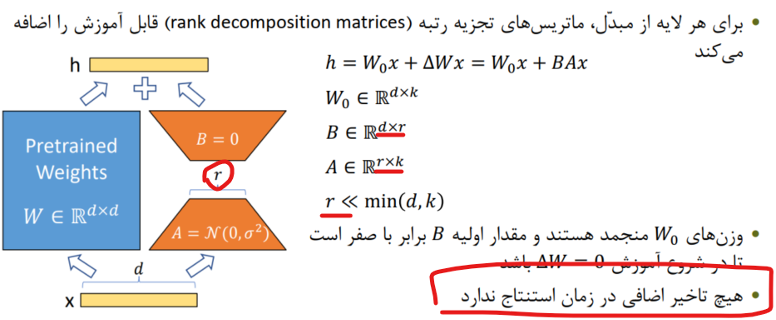
\includegraphics[width=\linewidth]{figs/image.png}
            \caption{محاسبه خروجی یک لایه \lr{LoRA}}
            \label{fig:q2_3}
        \end{figure}
        در مرحله استنتاج، تمام وزن‌ها ثابت هستند. از آنجایی که هم $W_0$ و هم ماتریس‌های آموزش‌دیده $B$ و $A$ ثابت هستند، می‌توان حاصل‌ضرب $BA$ را یک بار محاسبه کرد و با ماتریس اصلی ادغام نمود تا یک ماتریس وزن جدید ($W'$) به دست آید. این محاسبه فقط یک بار قبل از شروع به کار مدل (\lr{deployment}) انجام می‌شود. پس از آن، در زمان استنتاج، محاسبات به همان شکل مدل اصلی و بدون \lr{LoRA} انجام می‌شود. بنابراین، از آنجایی که محاسبات زمان اجرا دقیقاً معادل یک ضرب ماتریسی (مانند مدل اصلی) است، هیچ تأخیر محاسباتی اضافی وجود ندارد.\\
        \textbf{عدم وجود تأخیر اضافه در استنتاج.} زمانی که مدل در محیط عملیاتی به کار گرفته می‌شود، می‌توانیم به صورت صریح ماتریس $W = W_0 + BA$ را محاسبه و ذخیره کرده و استنتاج را مانند همیشه انجام دهیم. توجه داشته باشید که هر دو ماتریس $W_0$ و $BA$ در فضای $\mathbb{R}^{d \times k}$ قرار دارند. هنگامی که نیاز به تغییر به یک تسک پایین‌دستی دیگر داریم، می‌توانیم با کم کردن $BA$ از $W_0$، آن را بازیابی کرده و سپس یک ماتریس متفاوت $B'A'$ را به آن اضافه کنیم؛ این یک عملیات سریع با سربار حافظه بسیار ناچیز است.\\
        مرتبه یا رنک ($r$) در \lr{LoRA}، مستقیماً بر تعداد پارامترهای قابل آموزش و در نتیجه بر اندازه آداپتور \lr{LoRA} تأثیر می‌گذارد. رنک ($r$) بُعد میانی ماتریس‌های تجزیه‌شده $A$ و $B$ را تعیین می‌کند. این بدان معناست که:
        \begin{itemize}
            \item \textbf{رنک بالاتر (\lr{Higher Rank}):} تعداد پارامترهای قابل آموزش را افزایش می‌دهد. ظرفیت مدل برای یادگیری اطلاعات جدید و ویژه تسک را افزایش می‌دهد.
            \item \textbf{رنک پایین‌تر (\lr{Lower Rank}):} تعداد پارامترهای قابل آموزش را کاهش می‌دهد و مدل را بسیار بهینه‌تر می‌کند. ظرفیت مدل برای یادگیری را محدودتر می‌کند، که ممکن است برای تسک‌های پیچیده کافی نباشد.
        \end{itemize}
        بنابراین، رنک به عنوان یک ابرپارامتر (\lr{hyperparameter}) کلیدی عمل می‌کند که یک \textbf{\lr{trade-off}} بین کارایی پارامتری (\lr{parameter efficiency}) و قدرت مدل در حین فرآیند تنظیم دقیق (\lr{fine-tuning}) ایجاد می‌کند.\\}
        
        \item در تصویر زیر، یک معماری آداپتور برای شبکه‌های کانولوشنی نمایش داده شده است که ماژول "آداپتور" به‌ طور موازی با یک بلوک کانولوشنی (\lr{ConvBlock}) عمل می‌کند و خروجی آن به خروجی بلوک کانولوشنی اضافه می‌شود. در تصویر بعدی، هیستوگرام‌های \lr{feature map} های خروجی هر دو ماژول نشان داده شده‌اند. این هیستوگرام‌ها چه تفاوت‌هایی دارند و دلیل این تفاوت‌ها چیست؟ این تفاوت‌ها چه مشکلاتی می‌توانند ایجاد کنند و برای رفع این مشکلات چه راه‌حل‌هایی پیشنهاد می‌دهید؟ ( ۵ نمره)
        \begin{figure}[h]
            \centering
            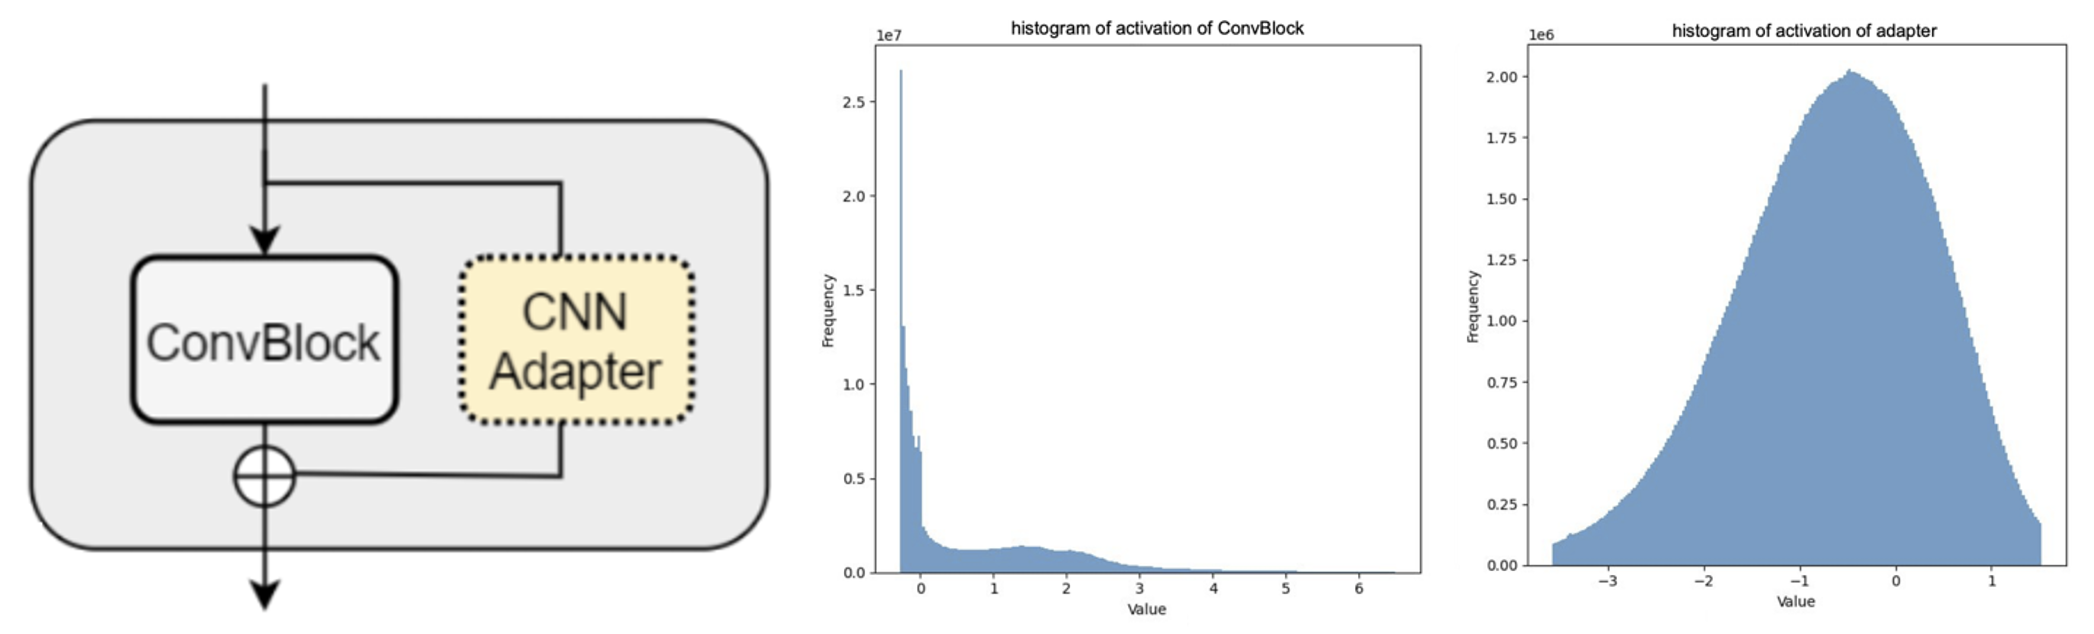
\includegraphics[width=\textwidth]{figs/Q2_4.png}
            \label{fig:q4}  
        \end{figure}

        \textcolor{blue}{
        هیستوگرام خروجی \lr{convblock} کاملاً نامتقارن و دارای چولگی به راست است. یک قله بسیار بزرگ و تیز در مقدار صفر وجود دارد و بقیه مقادیر در بازه مثبت پراکنده شده‌اند. درحالی که هیستوگرام ماژول آداپتور کاملاً متقارن است و شباهت زیادی به توزیع نرمال (گوسی) دارد. یکی از دلایل شکل هیستوگرام \lr{convblock} این است که این بلوک بخشی از یک شبکه از پیش‌آموخته است. وجود توابع فعال‌سازی مانند \lr{ReLU (Rectified Linear Unit)} پس از لایه‌های کانولوشنی، تمام مقادیر منفی را صفر می‌کند. این کار باعث ایجاد قله بزرگ در نقطه صفر و حذف مقادیر منفی می‌شود. وزن‌های این بلوک طی فرآیند آموزش روی داده‌های زیاد، به گونه‌ای تنظیم شده‌اند که ویژگی‌های معناداری استخراج کنند که منجر به چنین توزیع فعا‌ل‌سازی \lr{sparse} ای می‌شود. اما ماژول اداپتور به تازگی به شبکه اضافه شده و هنوز به طور کامل آموزش ندیده است. همچنین وزن‌های آداپتور معمولاً با مقادیر تصادفی کوچک و برگرفته از یک توزیع نرمال (با میانگین صفر) مقداردهی اولیه می‌شوند. در نتیجه، خروجی اولیه آن نیز شبیه به یک توزیع نرمال با میانگین صفر و واریانس پایین خواهد بود. این کار به این دلیل انجام می‌شود که در ابتدای آموزش، آداپتور نباید رفتار مدل از پیش‌آموخته را مختل کند. از سوی دیگر، ماژول آداپتور ممکن است از تابع فعال‌سازی متفاوتی مانند \lr{Tanh} استفاده کند یا حتی فاقد تابع فعال‌سازی محدودکننده باشد. این طراحی اجازه می‌دهد که مقادیر منفی در فعال‌سازی‌ها حفظ شوند و محدوده وسیع‌تری از مقادیر تولید شود. علاوه بر این، نقش ماژول آداپتور به عنوان یک مسیر مکمل در معماری شبکه به گونه‌ای است که ویژگی‌های متفاوتی نسبت به بلوک کانولوشنی استخراج می‌کند، که می‌تواند به پراکندگی بیشتر و توزیع نرمال‌مانند منجر شود.\\
        این تفاوت‌ها در توزیع فعال‌سازی‌ها می‌توانند هنگام جمع شدن خروجی‌های دو ماژول مشکلاتی ایجاد کنند. نخست، عدم تطابق در مقیاس و توزیع فعال‌سازی‌ها ممکن است باعث شود که یکی از ماژول‌ها بر دیگری غالب شود. برای مثال، اگر مقادیر ماژول آداپتور به دلیل پراکندگی بیشتر، دامنه وسیع‌تری داشته باشند، ممکن است تأثیر خروجی بلوک کانولوشنی را تحت‌الشعاع قرار دهند یا نویز ناخواسته‌ای به خروجی نهایی اضافه کنند. همچنین از آنجا که تأثیر اولیه آداپتور بر خروجی نهایی بسیار کم است، گرادیانی که برای به‌روزرسانی وزن‌های آن محاسبه می‌شود نیز بسیار کوچک خواهد بود (مشابه مشکل محو شدگی گرادیان یا \lr{Vanishing Gradient}). در نتیجه، فرآیند یادگیری آداپتور بسیار کند شده یا به درستی انجام نمی‌شود. هدف آداپتور، ایجاد تغییرات ظریف در رفتار مدل است. اگر خروجی آن در مقایسه با بلوک اصلی ناچیز باشد، مدل نمی‌تواند به طور مؤثری خود را با داده‌های جدید تطبیق دهد.\\
        \textbf{برای حل مشکل عدم تطابق مقیاس و اطمینان از آموزش مؤثر آداپتور، راه‌حل‌های زیر پیشنهاد می‌شود:}
        \begin{itemize}
            \item \textbf{استفاده از ضریب مقیاس‌پذیر:} این رایج‌ترین و مؤثرترین راه‌حل است. خروجی آداپتور قبل از جمع شدن با خروجی بلوک اصلی، در یک ضریب اسکالر $s$ ضرب می‌شود. این ضریب $s$ می‌تواند یک ابرپارامتر ثابت (مثلاً $s=2$) یا یک پارامتر قابل یادگیری باشد که به شبکه اجازه می‌دهد به طور خودکار بهترین مقیاس را برای خروجی آداپتور پیدا کند. این کار باعث تقویت سیگنال آداپتور شده و به آن اجازه می‌دهد تأثیر معناداری بر خروجی و فرآیند یادگیری بگذارد.
            \item \textbf{نرمال‌سازی لایه (\lr{Layer Normalization}):} می‌توان خروجی \lr{ConvBlock} را قبل از عملیات جمع، با استفاده از یک لایه نرمال‌سازی (مانند \lr{LayerNorm}) پردازش کرد. این کار باعث می‌شود خروجی بلوک اصلی دارای میانگین صفر و واریانس واحد شود و از نظر آماری به خروجی اولیه آداپتور نزدیک‌تر گردد.
        \end{itemize}
        }
    \end{enumerate}

    \item 
\includegraphics[width=1cm]{figs/Allowed_recommended.jpg}فرض کنید در حال کار روی یک پروژه طبقه‌بندی تصاویر پزشکی برای تشخیص یک بیماری نادر هستید. شما با دو چالش اصلی روبرو هستید:
        \begin{itemize}
            \item تعداد تصاویر برچسب‌خورده بسیار محدود است.
            \item مشخص نیست که چه نوع معماری شبکه‌ای برای این داده‌های خاص بهترین عملکرد را خواهد داشت.
        \end{itemize}
        با الهام از روش‌های معرفی شده در درس یک راهبرد\LTRfootnote{Strategy} جامع برای ساخت یک مدل طبقه‌بندی با کارایی بالا پیشنهاد دهید. در پاسخ خود به موارد زیر بپردازید(۱۵ نمره):
        \begin{itemize}
            \item برای انتخاب معماری، کدام رویکرد را انتخاب می‌کنید؟دلیل انتخاب خود را توضیح دهید.
            \item مزایا و معایب انتخاب شما در این شرایط خاص چیست؟
            \item چالش‌های اصلی در راهبرد پیشنهادی شما کدامند؟
        \end{itemize}

    \textcolor{blue}{
        \textbf{مرحله اول: انتخاب معماری شبکه}\\
        \textbf{رویکرد پیشنهادی:} استفاده از روش جستجوی معماری مانند \lr{DARTS} \LTRfootnote{Differentiable Architecture Search}.
        \begin{itemize}
            \item \textbf{عدم قطعیت در معماری:}  
            در حوزه‌های تخصصی مانند تصاویر پزشکی، معماری‌های استاندارد (که برای تصاویر طبیعی طراحی شده‌اند) لزوماً بهترین عملکرد را ندارند. ویژگی‌های بصری در تصاویر پزشکی (مانند بافت‌ها، مرزهای ظریف و کنتراست‌های خاص) ممکن است به ساختارهای متفاوتی در شبکه عصبی نیاز داشته باشند.
            \item \textbf{کارایی محاسباتی:}  
            چالش اصلی در پروژه‌های پزشکی، محدودیت منابع محاسباتی است. روش‌های جستجوی معماری مبتنی بر یادگیری تقویتی (\lr{RL}) یا الگوریتم‌های تکاملی، هزینه‌هایی معادل هزاران ساعت-\lr{GPU} دارند که آن‌ها را غیرعملی می‌سازد. در مقابل، \lr{DARTS} با هزینه جستجوی تنها ۱.۵ تا ۴ ساعت-\lr{GPU}، یک جایگزین بسیار کارآمد است که می‌تواند یک معماری بهینه و متناسب با داده‌های پزشکی موجود را کشف کند. این روش می‌تواند بلوک‌های سازنده (\lr{operations}) خاصی را کشف کند که برای استخراج ویژگی از این نوع تصاویر مناسب‌تر هستند.
            \item \textbf{جایگزین:}  
            اگر منابع محاسباتی برای اجرای \lr{DARTS} نیز فراهم نباشد، یک گزینه جایگزین خوب، استفاده از معماری \lr{DenseNet} است. این معماری به دلیل پارامترهای کمتر و استفاده مجدد از ویژگی‌ها (\lr{feature reuse}) شناخته شده و نشان داده است که در شرایط کمبود داده عملکرد بسیار خوبی دارد.
        \end{itemize}
        \textbf{مرحله دوم: استراتژی داده‌افزایی}\\
        \textbf{رویکرد پیشنهادی:} استفاده از \lr{Fast AutoAugment} برای کشف خودکار سیاست‌های داده‌افزایی.
        \begin{itemize}
            \item \textbf{مقابله با \lr{Overfitting}:}  
            با توجه به محدودیت شدید داده‌ها، داده‌افزایی برای جلوگیری از بیش‌برازش (\lr{Overfitting}) و بهبود تعمیم‌پذیری مدل حیاتی است.
            \item \textbf{نیاز به داده‌افزایی تخصصی:}  
            داده‌افزایی در تصاویر پزشکی بسیار حساس است. یک چرخش یا تغییر رنگ شدید که برای تصاویر طبیعی بی‌خطر است، می‌تواند معنای تشخیصی یک تصویر پزشکی را کاملاً تغییر دهد. برای مثال، برعکس کردن افقی یک تصویر رادیوگرافی قفسه سینه می‌تواند موقعیت قلب را جابجا کرده و منجر به تشخیص اشتباه شود. بنابراین، تعیین دستی پارامترهای مناسب (مانند حداکثر زاویه چرخش یا میزان تغییر کنتراست) دشوار و نیازمند تخصص پزشکی است.
            \item \textbf{راه‌حل خودکار و کارآمد:}  
            \lr{Fast AutoAugment} این مشکل را با جستجوی خودکار در فضای پارامترهای داده‌افزایی حل می‌کند. با تعریف یک فضای جستجوی اولیه شامل عملیات‌های ``امن'' برای تصاویر پزشکی (مانند چرخش‌های جزئی، تغییرات کنتراست و روشنایی محدود، و تغییر شکل‌های الاستیک)، این الگوریتم می‌تواند بهترین ترکیب، احتمال و شدت این عملیات‌ها را به صورت خودکار و متناسب با داده‌های موجود پیدا کند. هزینه محاسباتی پایین آن نیز این روش را برای این سناریو کاملاً عملی می‌سازد.
        \end{itemize}
        \textbf{چالش‌ها}
        \begin{itemize}
            \item \textbf{هزینه در مقابل دقت:}  
            با وجود کارایی بالا، ترکیب \lr{DARTS} و \lr{Fast AutoAugment} همچنان از آموزش یک مدل استاندارد روی داده‌های موجود پرهزینه‌تر است. این یک بده‌بستان بین سرمایه‌گذاری محاسباتی اولیه برای جستجو و دقت بالقوه بالاتر در مدل نهایی است.
            \item \textbf{نمایندگی داده‌ها:}  
            موفقیت این استراتژی به شدت به این وابسته است که مجموعه داده محدود اولیه، نماینده خوبی از توزیع واقعی داده‌های آن بیماری باشد. اگر داده‌های اولیه سوگیرانه (\lr{biased}) باشند، معماری و سیاست‌های کشف‌شده نیز بهینه نخواهند بود.
            \item \textbf{نیاز به تعریف فضای جستجوی اولیه:}  
            اگرچه فرآیند جستجو خودکار است، اما تعریف فضای عملیات اولیه برای داده‌افزایی نیازمند مقداری دانش دامنه است تا از اعمال تبدیلات نامعتبر از نظر پزشکی جلوگیری شود.
        \end{itemize}
    }
        
    \item 
\includegraphics[width=1cm]{figs/Allowed_recommended.jpg}\lr{Fast AutoAugment} به عنوان یک راهکار برای رفع مشکل اصلی \lr{AutoAugment}، یعنی هزینه محاسباتی بالا، معرفی شده است. با توجه به الگوریتم و توضیحات ارائه شده در درس، به سوالات زیر پاسخ دهید(۱۵ نمره):
    \begin{enumerate}
        \item ایده کلیدی پشت \lr{Fast AutoAugment} که آن را سریع‌تر می‌کند، چیست؟ مفهوم 
تطابق چگالی\LTRfootnote{Density Matching} را توضیح دهید.
        \item استراتژی تقسیم داده‌ها به \lr{K-fold} و استفاده از مجموعه‌های $D_{\mathcal{A}}^{(k)}, D_{\mathcal{M}}^{(k)}$ چگونه به کاهش هزینه محاسباتی کمک می‌کند؟
        \item با استفاده از جدول مقایسه هزینه محاسباتی ، تفاوت سرعت این روش با \lr{AutoAugment} را برای مجموعه داده \lr{ImageNet} به صورت کمی بیان کرده و اهمیت این بهبود را تحلیل کنید.
    \end{enumerate}

    \textcolor{blue}{
        روش \lr{Fast AutoAugment} برای حل بزرگ‌ترین نقطه ضعف \lr{AutoAugment}، یعنی هزینه محاسباتی بسیار بالا، طراحی شد. این بهبود از طریق یک نوآوری کلیدی در استراتژی جستجو و یک رویکرد هوشمندانه برای ارزیابی سیاست‌های داده‌افزایی به دست آمده است.
        \begin{itemize}
            \item \textbf{الف) ایده کلیدی: تطابق چگالی}\\
            ایده اصلی و نوآورانه در \lr{Fast AutoAugment}، جایگزین کردن هدف جستجو است. در حالی که \lr{AutoAugment} اصلی سعی می‌کرد سیاستی را پیدا کند که دقت مدل را در مجموعه اعتبارسنجی بیشینه کند (فرآیندی که نیازمند آموزش کامل یک مدل برای هر سیاست بود)، \lr{Fast AutoAugment} هدف متفاوتی را دنبال می‌کند: پیدا کردن سیاست‌های داده‌افزایی که توزیع داده‌های افزایش‌یافته را به توزیع داده‌های اصلی نزدیک‌تر کنند.  
            این ایده با عنوان ``تطابق چگالی'' یا ``همخوانی توزیع'' شناخته می‌شود. منطق پشت این ایده این است که یک سیاست داده‌افزایی ``خوب''، داده‌های جدیدی تولید می‌کند که از نظر آماری شبیه به داده‌های واقعی مجموعه آموزشی هستند و مدل را سردرگم نمی‌کنند.  
            این رویکرد به الگوریتم اجازه می‌دهد تا کیفیت یک سیاست داده‌افزایی را بدون نیاز به اجرای یک فرآیند آموزش کامل و پرهزینه، سریع و کارآمد ارزیابی کند. به جای یادگیری تقویتی، این روش از \lr{Bayesian Optimization} برای جستجوی کارآمد در فضای پیوسته پارامترهای داده‌افزایی استفاده می‌کند.
            \item \textbf{ب) نقش استراتژی \lr{K-fold} در کاهش هزینه محاسباتی}\\  
            \begin{itemize}
                \item \textbf{تقسیم \lr{K-fold}:} ابتدا، مجموعه داده آموزشی $D_{train}$ به $K$ بخش تقسیم می‌شود. این کار به الگوریتم اجازه می‌دهد تا جستجو را به صورت موازی روی بخش‌های مختلف داده انجام دهد.  
                \item \textbf{تقسیم داخلی:} هر بخش خود به دو زیرمجموعه تقسیم می‌شود:  
                \begin{itemize}
                    \item $D_{M}^{(k)}$: بخشی از داده‌ها که برای آموزش یک مدل پایه $M(\theta)$ استفاده می‌شود.  
                    \item $D_{A}^{(k)}$: بخشی دیگر که برای ارزیابی سیاست‌های داده‌افزایی به کار می‌رود.  
                \end{itemize}
                \item \textbf{یک بار آموزش، ارزیابی چندباره:} مدل پایه $M(\theta)$ برای هر \lr{fold} فقط یک بار روی $D_{M}^{(k)}$ آموزش می‌بیند. سپس، تعداد زیادی $(B)$ سیاست داده‌افزایی روی $D_{A}^{(k)}$ با استفاده از همین مدلِ از قبل آموزش‌دیده ارزیابی می‌شوند.  
            \end{itemize}
            این استراتژی، گلوگاه محاسباتی \lr{AutoAugment} اصلی را از بین می‌برد، زیرا دیگر نیازی نیست که به ازای هر سیاست کاندید، یک مدل از ابتدا تا انتها آموزش داده شود.
            \item \textbf{ج) مقایسه کمی هزینه محاسباتی}\\  
            تفاوت در کارایی این دو روش در مقایسه مستقیم هزینه‌های محاسباتی آن‌ها مشهود است.  
            \begin{itemize}
                \item \lr{AutoAugment}: ۱۵۰۰۰ ساعت-\lr{GPU}  
                \item \lr{Fast AutoAugment}: ۴۵۰ ساعت-\lr{GPU}  
            \end{itemize}
            این اعداد نشان‌دهنده یک کاهش هزینه بیش از ۳۳ برابر است. این بهبود چشمگیر، تکنیک جستجوی خودکار داده‌افزایی را از یک پروژه تحقیقاتی بسیار گران‌قیمت که تنها در توان شرکت‌های بزرگ بود، به ابزاری عملی و قابل دسترس برای جامعه گسترده‌تری از محققان و توسعه‌دهندگان تبدیل کرده است.
        \end{itemize}
    }


   
    
    \section*{سوالات عملی} 
    \item 
\includegraphics[width=1cm]{figs/Allowed_with_contributino.jpg}
    در این تمرین، قصد داریم فرآیند بهینه‌سازی یک شبکه عصبی را به صورت عملی تجربه کنیم. این فرآیند با ساخت یک مدل پایه  آغاز شده و با پیاده‌سازی و مقایسه طیف وسیعی از تکنیک‌های بهینه‌سازی هایپرپارامتر، از روش‌های کلاسیک مانند جستجوی شبکه‌ای تا الگوریتم‌های پیشرفته مانند \lr{Optuna} با قابلیت هرس کردن و الگوریتم ژنتیک، ادامه می‌یابد.
    وظیفه اصلی شما، تکمیل بخش‌های مشخص‌شده در نوت‌بوک \lr{HyperparameterOptimization.ipynb} است. در نهایت، از شما خواسته می‌شود تا نتایج روش‌های مختلف را تحلیل کرده و کارایی و عملکرد آن‌ها را با یکدیگر مقایسه نمایید(۳۰ نمره).

    \textcolor{blue}{\textbf{لطفا به فایل \lr{hyperparameteroptimization-answer.ipynb} مراجعه نمایید.}}




    
 
\end{enumerate}



\end{document}


